\chapter{Протокол WEP}

WiFi сети можно разделить на два типа по методу аутентификации: открытая
аутентификация и аутентификация с общим ключом. Для сетей с аутентификацией с
общим ключом существует несколько алгоритмов для обеспечения безопасности: Wired
Equivalent Privacy (WEP), Wi-Fi Protected Access (WPA, WPA2).

\section{Общие сведения о WEP}

WEP --- протокол обеспечения безопасности беспроводных сетей WiFi. Используется
для обеспечения конфиденциальности и защиты передаваемых данных авторизованных
пользователей беспроводной сети от прослушивания.  Существует две разновидности
WEP: WEP-40 и WEP-104, различающиеся только длиной ключа. В настоящее время
данная технология является устаревшей, так как ее взлом может быть осуществлён
всего за несколько минут. Тем не менее, она продолжает широко использоваться.

В 1997 году IEEE одобрил механизм WEP. В октябре 2000-го года вышла статья
Джесси Уолкера «Unsafe at any key size; An analysis of the WEP encapsulation»,
описывающая проблемы алгоритма WEP и атаки, которые могут быть организованы с
использованием его уязвимостей.  В алгоритме есть множество слабых мест:

\begin{itemize}
    \item механизмы обмена ключами и проверки целостности данных;
    \item малая разрядность ключа и вектора инициализации;
    \item способ аутентификации;
    \item алгоритм шифрования.
\end{itemize}

В 2001 году появилась спецификация WEP-104, которая, тем не менее, не решила
проблемы, так как длина вектора инициализации и способ проверки целостности
данных остались прежними. В 2004 году IEEE одобрил новые механизмы WPA и WPA2. В
2008 году совет Payment Card Industry Security Standards Council обновил
стандарт безопасности данных индустрии платёжных карт, в котором запретили
использовать протокол WEP во всех этапах обработки кредитных карт после 30 июня
2010 года, а также запретили использование протокла WEP во всех новых системах с
31 марта 2009 года.

В основе WEP лежит поточный шифр RC4, выбранный из-за своей высокой скорости
работы и возможности использования переменной длины ключа. Для подсчёта
контрольных сумм используется CRC32.

Кадр WEP включает в себя следующие поля:
\begin{enumerate}
    \item Незашифрованная часть:
    \begin{itemize}
        \item вектор инициализации (24 бита);
        \item пустое место (6 бит);
        \item идентификатор ключа (2 бита).
    \end{itemize}
    \item Зашифрованная часть:
    \begin{itemize}
        \item данные;
        \item контрольная сумма (32 бита).
    \end{itemize}
\end{enumerate}

\section{Алгоритм поточного шифрования RC4}

В протоколе WEP используется поточный алгоритм шифрования RC4. Ключом для RC4
является вектор инициализации и собственно общий ключ WEP. Таким образом 3 байта
вектора инициализации и 5 или 13 байт ключа WEP составляют, соответственно, 8
или 16 байт ключа RC4 [5].

Основные преимущества шифра --- высокая скорость работы и переменный размер
ключа. RC4 довольно уязвим, если используются не случайные или связанные ключи,
один ключевой поток используется дважды. Эти факторы, а также способ
использования могут сделать криптосистему небезопасной. Алгоритм инициализации
RC4 приведён ниже. Этот алгоритм также называется алгоритмом ключевого
расписания (KSA), см. рис.~\ref{fig:array_initialization_scrembling}.
Этот алгоритм использует ключ, сохранённый в Key, и имеющий длину L байт.
Инициализация начинается с заполнения массива S, далее этот массив
перемешивается путём перестановок, определяемых ключом. Так как только одно
действие выполняется над S, то должно выполняться утверждение, что S всегда
содержит все значения кодового слова.

\begin{figure}
    \begin{lstlisting}
    for i = 0 to 2n - 1
        S[i] = i
    j = 0
    for i = 0 to 2n - 1
        j = (j + S[i] + Key[i mod L]) mod 2n
        Перестановка(S[i], S[j])
    \end{lstlisting}
    \caption{Начальное заполнение массива и скремблирование}
    \label{fig:array_initialization_scrembling}
\end{figure}

Генератор ключевого потока RC4 переставляет значения, хранящиеся в S, и каждый
раз выбирает различное значение из S в качестве результата. В одном цикле RC4
определяется одно n-битное слово K из ключевого потока, которое в последующем
суммируется с исходным текстом для получения зашифрованного текста. Эта часть
алгоритма называется генератором псевдослучайной последовательности (PRGA).

В отличие от современных шифров, RC4 не использует отдельного случайного числа
(nonce) наряду с ключом. Это значит, что если один ключ должен использоваться в
течение долгого времени для шифрования нескольких потоков, сама криптосистема,
использующая RC4, должна комбинировать случайное число и долгосрочный ключ для
получения потокового ключа для RC4. Один из возможных выходов --- генерировать
новый ключ для RC4 с помощью хэш-функции от долгосрочного ключа и случайного
числа.  Однако, многие приложения, использующие RC4, просто конкатенируют ключ и
случайное число.  Из-за этого и слабого расписания ключей, используемого в RC4,
приложение может стать уязвимым.

\subsection{Исследования Руза и восстановление ключа из перестановки}

В 1995 году Андрю Руз (Andrew Roos) экспериментально пронаблюдал, что первый
байт ключевого потока коррелирован с первыми тремя байтами ключа, а первые
несколько байт перестановки после алгоритма расписания ключей (KSA)
коррелированы с некоторой линейной комбинацией байт ключа [6]. Эти смещения не
были доказаны до 2007 года, когда Пол, Рафи и Мэйтрэ доказали коррелированность
ключа и ключевого потока [7]. Также Пол и Мэйтрэ доказали коррелированность
перестановки и ключа [8]. Последняя работа также использует коррелированность
ключа и перестановки для того, чтобы создать первый алгоритм полного
восстановления ключа из последней перестановки после KSA, не делая предположений
о ключе и векторе инициализации. Этот алгоритм имеет постоянную вероятность
успеха в зависимости от времени, которая соответствует квадратному корню из
сложности полного перебора.

Позднее было сделано много работ о восстановлении ключа из внутреннего состояния RC4.

\subsection{Атака Флурера, Мантина и Шамира (FMS)}

В 2001 году, Флурер, Мантин и Шамир опубликовали работу об уязвимости ключевого
расписания RC4 [3]. Они показали, что среди всех возможных ключей, первые несколько
байт ключевого потока являются совсем неслучайными. Из этих байт можно с высокой
вероятностью получить информацию о используемом шифром ключе. И если
долговременный ключ и случайное число просто конкатенируются для создания ключа
шифра RC4, то этот долговременный ключ может быть получен с помощью анализа
достаточно большого количества сообщений, зашифрованных с использованием данного
ключа. Эта уязвимость и некоторые связанные с ней эффекты были использованы
при взломе шифрования WEP в беспроводных сетях стандарта IEEE 802.11. Это
показало необходимость скорейшей замены WEP, что повлекло за собой разработку
нового стандарта безопасности беспроводных сетей WPA.

Криптосистему можно сделать невосприимчивой к этой атаке, если отбрасывать
начало ключевого потока. Таким образом модифицированный алгоритм называется
«RC4-drop[n]», где n --- количество байт из начала ключевого потока, которые
следует отбросить. Рекомендовано использовать n = 768, консервативная оценка
составляет n = 3072.

\subsection{Комбинаторная проблема}

В 2001 году Ади Шамир и Ицхак Мантин первыми поставили комбинаторную проблему,
связанную с количеством всевозможных входных и выходных данных шифра RC4. Если
из всевозможных 256 элементов внутреннего состояния шифра известно x элементов
из состояния ($x \le 256$), то, если предположить, что остальные элементы нулевые,
максимальное количество элементов, которые могут быть получены детерминированным
алгоритмом за следующие 256 раундов также равно x. В 2004 году это предположение
было доказано Сорадюти Полом (Souradyuti Paul) и Бартом Прэнилом (Bart Preneel) [9].


\subsection{Атака Кляйна}

В 2005 году Андреас Кляйн представил анализ шифра RC4, в котором он указал на
сильную коррелированность ключа и ключевого потока RC4 [10]. Кляйн
проанализировал атаки на первом раунде (подобные атаке ФМШ), на втором раунде и
возможные их улучшения. Он также предложил некоторые изменения алгоритма для
усиления стойкости шифра. В частности, он утверждает, что если поменять
направление цикла на обратное в алгоритме ключевого расписания, то можно сделать
шифр более стойким к атакам типа ФМШ.

\section{Пример шифрования RC4 фиксированных входных данных WEP}

Для отправки сообщения в сети с протоколом WEP отправитель должен сгенерировать
вектор инициализации и у него должен быть ключ WEP и данные, которые он
собирается отправить. Рассмотрим процесс шифрования на примере отправки
ARP-ответа, исходный код представлен в приложении~\ref{app:rc4}, результат работы
данного кода отображён на рисунке~\ref{fig:rc4_encrypt_example}.

\begin{figure}
    \centering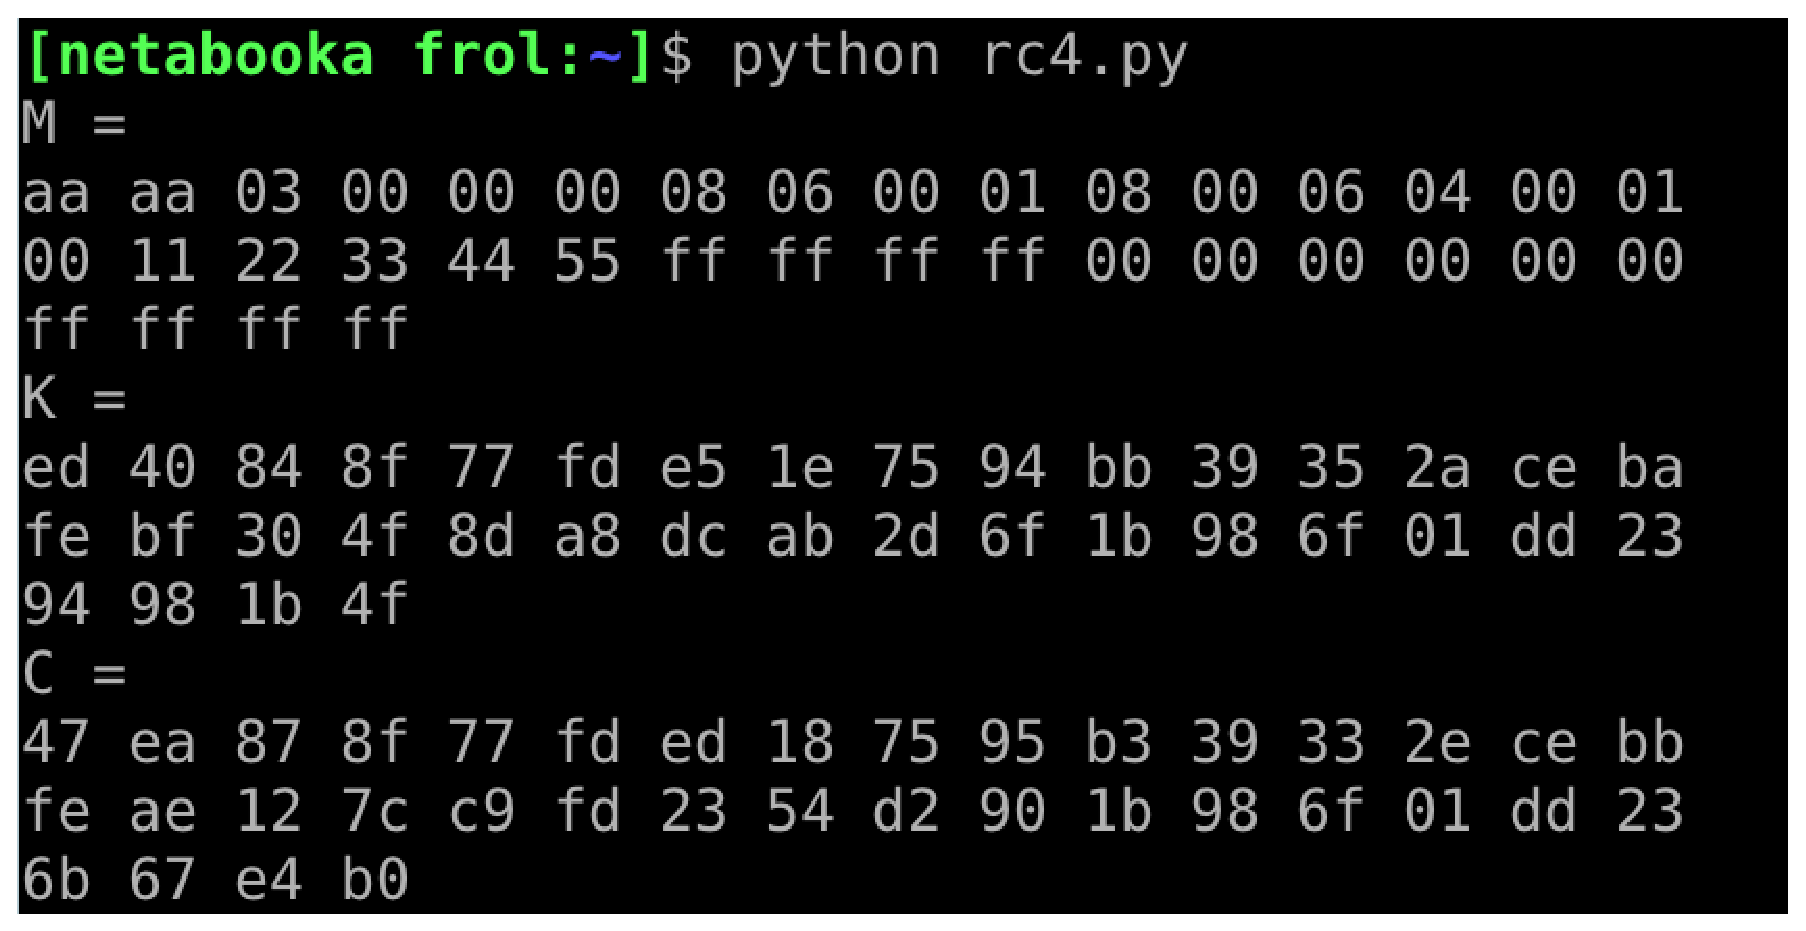
\includegraphics[width=0.8\textwidth]{graphics/rc4_encrypt_example.eps}
    \caption{Результат шифрования RC4 на примере\\ ARP-ответа в WEP}
    \label{fig:rc4_encrypt_example}
\end{figure}
